\documentclass[12pt,titlepage]{article}

\usepackage{ngerman,amsmath,graphicx, a4wide}

\begin{document}

\title{Miniprojekt: \\ Minimax-Maschine}
\author{Clemens Pollak, Robin Thrift, Max Boll}
\date{2014}
\maketitle


\section{Einleitung} 
Unser gew{\"a}hltes Thema befasst sich mit der Minimax-Maschine und mit der Realisierung von Algorithmen auf ihr. Dieses Thema soll im Rahmen des Hardware Praktikums bearbeitet werden und ist uns aus der Veranstaltung "'Grundlagen der Rechnerarchitektur"' bereits grundlegend bekannt.\\ Um unsere Vorbereitung auf dieses Projekt dokumentieren und strukturieren zu k{\"o}nnen, erstellen wir ein Pflichtenheft. Dieses Pflichtenheft wird nur unsere Vorbereitung beinhalten und es wird au{\ss}erdem eine weitere Dokumentation der Ergebnissen geben. Außerdem wird es w{\"a}hrend der Bearbeitung unseres Projects einen Leitfaden führ uns darstellen, der die Implementierung der L{\"o}sung vereinfacht und beschleunigt.

\section{Aufgabenstellung}
Nach unserem Verst{\"a}ndniss ist das Ziel dieser Aufgabenstellung einen Algorithmus, welcher auf der Minimax-Maschine zu implementieren ist und eine sogenannte Paketanalyse betreibt. Dieser "'Paketanalyse"'-Algorithmus befasst sich mit dem Datenpaketen, welche im Speicher der Minimax-Maschine abgelegt sind.\\ Ein Datenpaket beginnt immer mit der Folge "'1110"' und besteht aus einem
Kopf mit einer L{\"a}nge von 80 Bits und einem Datenteil mit variabler L{\"a}nge. Der Kopf enth{\"a}lt die Kanalnummer zwischen der 32. und 47. Bitstelle. Zu einem Kanal k{\"o}nnen ein oder mehrere Pakete geh{\"o}ren, welche die selbe Kanalnummer haben.
Die L{\"a}nge des kompletten Paketfeldes im Speicher wird als bekannt vorausgesetzt. Deswegen werden die einzelnen L{\"a}ngen der Pakete in ein entsprechendes Register vorgeladen.\\
Nun soll der Algorithmus eine Datentabelle anlegen, welche sich au{\ss}erhalb der Speicherfelder der einzelnen Pakete befindet. Diese Datentabelle soll den Kanalnummern die L{\"a}ngen der jeweiligen Datenteile aller Pakete zuordenen um dann später exportiert zu werden. Diese Aufgabenstellung soll mit dem Minimax-Simulator simuliert und getestet werden. Die Maschine kann durch vorgegebene Bauteile erweitert werden, was sich aber auf die Bewertung auswirkt. Der Algorithmus wird in Form der sogenannten Steuertabelle implementiert und soll außerdem als Flussdiagramm abgegeben werden.


\section{Ist-Analyse der Basis-Maschine}

Die Minimax-Maschine ist ein minimales Rechensystem welches aus einfachen Registern (Basis: \texttt{ACCU}, \texttt{PC}, \texttt{IR}, \texttt{MDR}, \texttt{MAR};
weitere k{\"o}nnen hinzuge{\"u}fgt werden), einer arithmetisch-logischen Einheit (ALU) und einem Hauptspeicher (HS) aufgebaut
ist und durch ein Mikropgramm gesteuert wird. Jedes dieser Register hat als Eingang mindestens die ALU und hat zusätzlich einen Eingang, der den Schreibzugriff regelt.\\
\\
\\
\begin{enumerate}
\item \texttt{ACCU}: Abk{\"u}rzung f{\"u}r "'Accumulator"' ein Zwischenspeicher, um mit \texttt{MDR} Operationen durchführen zu k{\"o}nnen.
\item \texttt{PC}: Abk{\"u}rzung f{\"u}r "'program counter"', wird meistens f{\"u}r das Z{\"a}hlen bzw. erh{\"o}en einer Speicheradresse benutzt.
\item \texttt{IR}: Abk{\"u}rzung f{\"u}r "'instruction register"', enthält Opcode(8 Bit) und Adressteil(24 bit).
\item \texttt{MDR}: Abk{\"u}rzung f{\"u}r "'memory data register"', enthält je nach Einstellung des Multiplexers texttt{MDR.Sel}, verschiede Daten entweder aus Hauptspecher oder aus der \texttt{ALU}.
\item \texttt{MAR}: Abk{\"u}rzung f{\"u}r "'memory adress register"', enth{\"u}lt die Speicheradresse an der aus dem Hauptspeicher Daten geladen oder geschrieben werde sollen.
\item \texttt{HS}: Abk{\"u}rzung f{\"u}r "'Hauptspeicher"', er wird mit 24-Bit durch \texttt{MAR} adressiert und gibt eine 32-Bit Zahl zur{\"u}ck. Auf die selbe Art funktioniert schreiben einer 32-Bit Zahl nat{\"u}rlich auch.
\end{enumerate}
Dabei sind die m{\"o}glichen Operationen auf die in der ALU implementieren
Operationen beschr{\"a}nkt (Basis: \texttt{ADD}, \texttt{SUB.B}, \texttt{TRANS.A}, \texttt{TRANS.B}). Die ALU kannn mit weiteren Operationen,
wie z. B. dem bitweisen UND, erg{\"a}nzt werden.\\
Um eine Operation auszuf{\"u}hren m{\"u}ssen {\"u}ber die Multiplexer \texttt{ALUSel.A} und \texttt{AluSel.B} zwei Operanden ausgew{\"a}hlt werden
und der ALU muss {\"u}ber die \texttt{ALU Ctrl}-Leitung der Code f{\"u}r die Operation {\"u}bergben werden. An den Multiplexern liegen sowohl
Konstanten als auch die Register an, welche zur ALU durchgeschaltet werden k{\"o}nnen. Das Ergebnis der Operation kann
entweder in einem Register oder im HS (Adresse im Register \texttt{MAR}) gespeichert werden. Zus{\"a}tzlich k{\"o}nnen s. g. Flags 
gesetzt werden, welche zur{\"u}ck zur Control Unit (CU) geleitet werden um z. B. bedingte Spr{\"u}nge auszuf{\"u}hren.


Die uns vorliegende Minimax-Maschine arbeitet mit 32-Bit und speichert Werte mit 32-Bit in den Registern und im HS.
Alle ALU-Operationen werden folglich alle mit 32-Bit ausgef{\"u}hrt. Dies stellt sich jedoch f{\"u}r unser Aufgabe als
Hindernis, da wir die Daten bitweise untersuchen m{\"u}ssen, Daten aus dem HS und den Registern jedoch nur als
32-Bit Zahlen auslesen k{\"o}nnen und nicht als einzelne Bits.

Folglich wird die Basismaschine um einige Konstanten, Operationen und Register erweitert werden müssen, welche im "'Implementierungskonzept'" n{\"a}her
aufgeführt sind.


\section{Implementierungskonzept}
Die vorliegende Aufgabenstellung kann in mehrere Teilprobleme zerlegt werden:
\begin{enumerate}
\item Das sequenzielle Auslesen des Hauptspeichers
\item Die Analyse der Daten
    \begin{enumerate}
    \item Das erkennen der Startsequenz eines neuen Pakets
    \item Das Auslesen der Kanalnummer
    \end{enumerate}
\item Das speichern der geforderten Daten im HS
\end{enumerate}

\subsection{Sequenzielles Auslsesen aus dem Hauptspeicher}
Zun{\"a}chst m{\"u}ssen also die abgelegten sequenziell Daten ausgelsen werden. Hierzu wird ein Mirkoprogramm implementiert, welches mithilfe
einer Schleife alle Speicherzellen ausliest, bis es auf eine nicht initialisierte (Wert = 0) Speicherzelle trifft. 
Hierzuh muss die Minimax-Maschine um ein Register erweitert werden welches die akutelle Speicheradresse enth{\"a}lt (anfangs 0),
und mit wir \texttt{ADDR} bezeichnen werden. Bei jeder Iteration wird der Wert an der Adresse \texttt{ADDR} im Register 
\texttt{MDR} gespeichert und steht somit dem Analyseprogramm zur verf{\"u}gung. Nach der Analyse wird das Register \texttt{ADDR}
inkrementiert und es wird zur{\"u}ck zum Schleifenkopf gesprungen (Siehe Abb. 1 im Anhang).

\subsection{Analyse der Daten}


Wie bereits in der Ist-Analyse beschrieben handelt es sich um eine 32-Bit Maschine welche Daten als 32-Bit-Zahlen behandelt und nicht als 
einzelne Bits. Dies erschwert die Suche nach der Anfangssequenz der Datenpakete ($1110_{2} = 14_{10}$). Um diese Sequenz in der 32-Bit-Zahl
zu finden muss mit diesem Muster also Maskiert werden. Dies geschieht {\"u}ber die bitweise Und-Verkn{\"u}pfung mit dem Muster. F{\"u}r die Minimax-Maschine
heißt das konkret: 14 \& ZAHL bitweise Und-verkn{\"u}pfen. Folglich wird die Basismaschine um die Konstante 14 ($=1110_{2}$) und eine bitweise UND-Operation
erweitert.\\
Die Tabelle die als Ergebnis erstellt werden soll (siehe n{\"a}chster Abschnitt) kann nach erkennen der Anfangssequenz erstellt werden:
Durch {\"u}berspringen der ersten 32 irrelevanten Bits wird die 15 Bit lange Kanalnummer ausgelesen und gespeichert. Dazu wird die in einem Register liegende l{\"a}nge des Datenpacketes geschrieben. Dieser Vorgang wiederholt sich.\\
Eine genaue Implementierung kann anhand eines Flow-Diagramms in RT-Notation im Anhang nachvollzogen werden.


\section{Angestrebte Projektergebnisse}
\begin{enumerate}
\item Die Tabelle, in der die einzelnen Kanalnummern und Paketl{\"a}ngen enthalten sind. (Als exportierte Speicherdatei)
\item Eine Dokumentation, welche unserer Implementierung im Detail beschreibt und m{\"o}glicherweise schwierige Stellen verst{\"a}ndlich erl{\"a}utert.
\item Einen exportierten Schaltplan der erweiterten Minimax-Maschine.
\end{enumerate}

\section{Anhang mit Flussdiagrammen \\ geplanter Mikroprogramme}

\subsection{Abb. 1: Flussdiagramm des Speicherauslesepgrogramms}

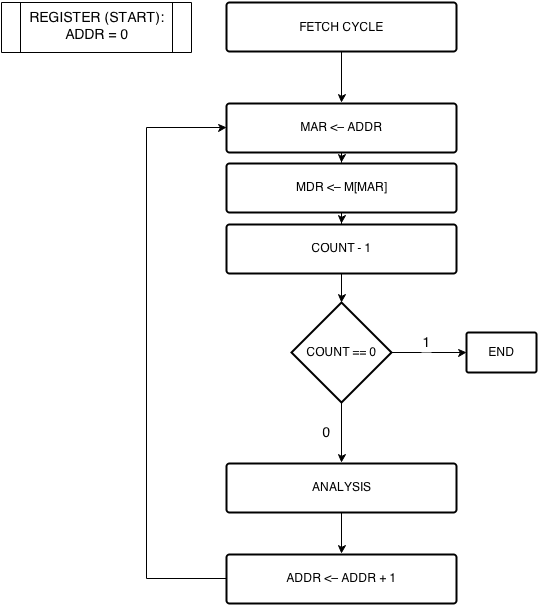
\includegraphics[width=13cm]{readFromMemory.png}

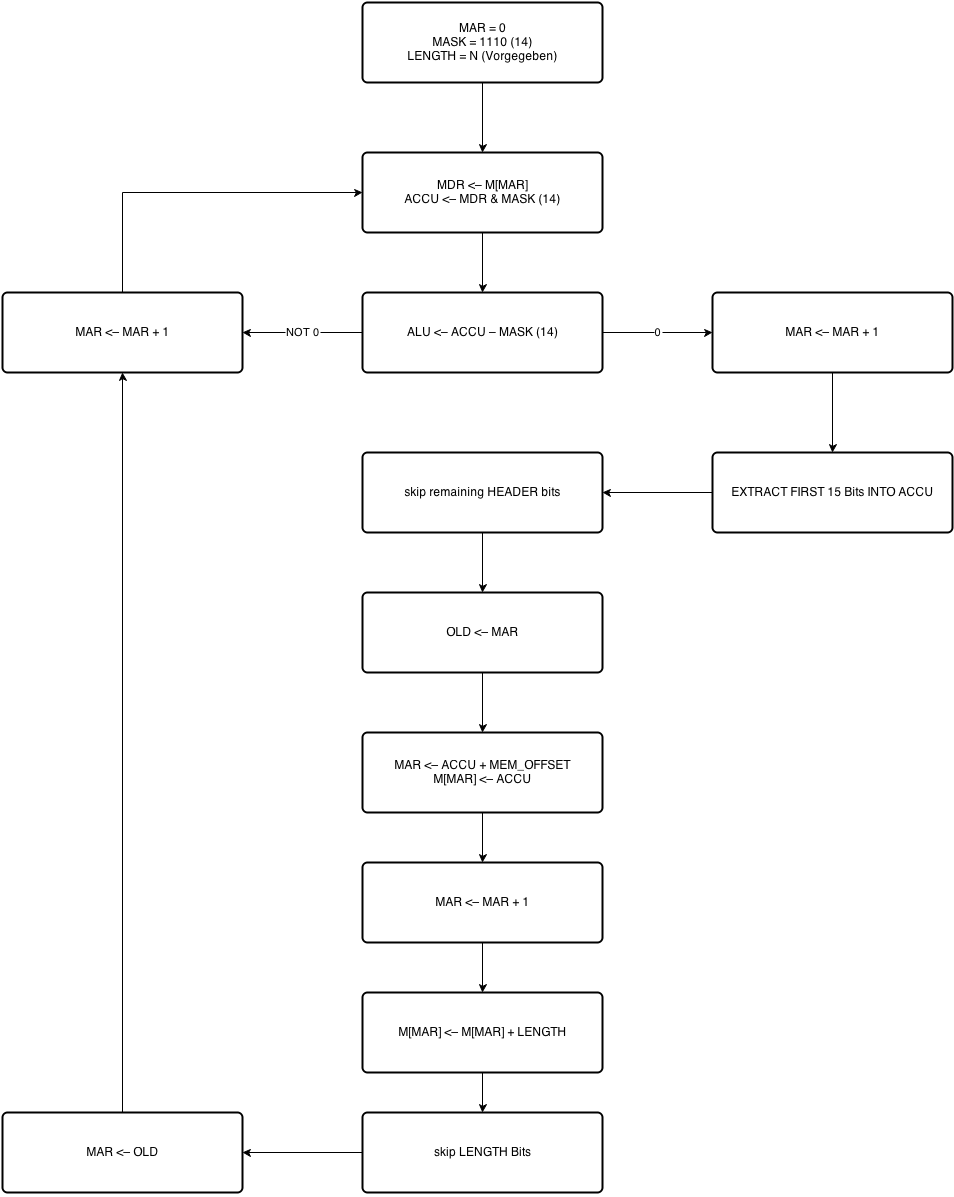
\includegraphics[width=13cm]{algo_flow.png}

\section{Arbeitsaufteilung}

\begin{tabular} { |l||c| }
\hline
Robin Thrift & Aufgabe1 \\
\hline
Clemens Pollak & Aufgabe1 \\
\hline
Max Boll & Aufgabe1 \\
\hline
\end{tabular}

\section{Hilfsmittel}
Wir haben folgende Quellen benutzt:
\begin{enumerate} 
\item Internet (wikipedia.de, github.com)
\item Der SRA Minimax-Simulator
\item Informationsfolien (Aufgabenstellung)
\item Die Grundlagen der Rechnerarchitektur Materialien
\end{enumerate}

\end{document}
